\begin{figure}[htb]
    \begin{subfigure}{0.35\linewidth}
        \centering
        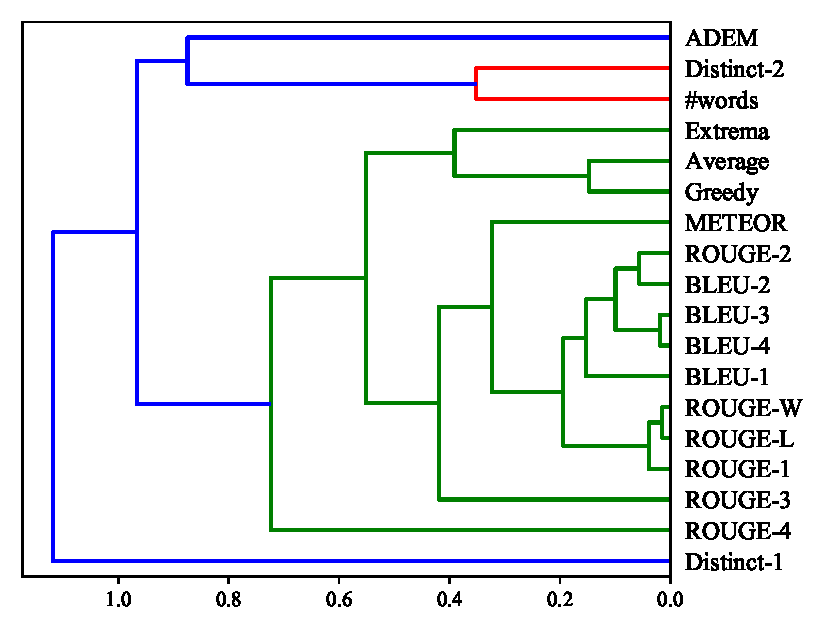
\includegraphics[width=\linewidth]{figure/plot/hierarchy/v3/pearson/hred/lsdscc/plot.pdf}
        \caption{(HRED, LSDSCC)}
    \end{subfigure}%
    \begin{subfigure}{0.35\linewidth}
        \centering
        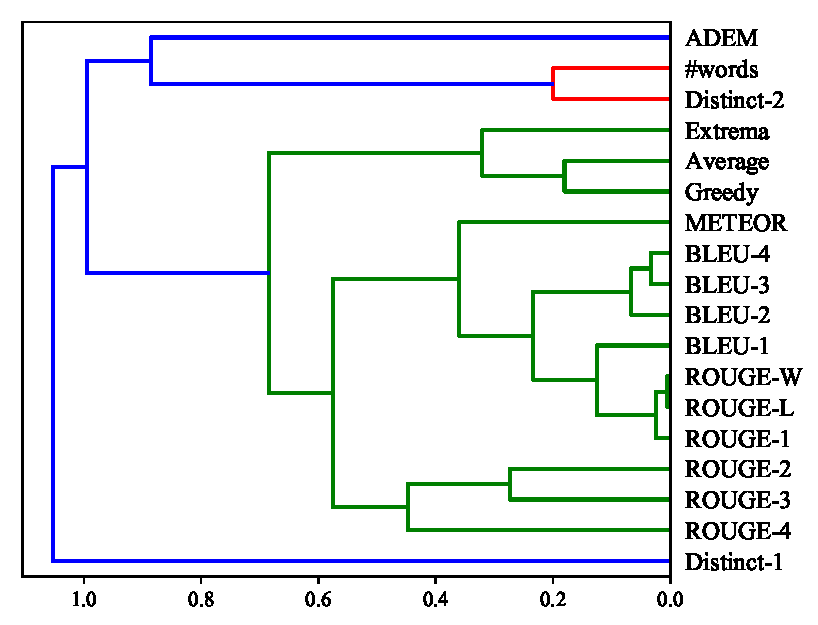
\includegraphics[width=\linewidth]{figure/plot/hierarchy/v3/pearson/hred/opensub/plot.pdf}
        \caption{(HRED, OpenSubtitles)}
    \end{subfigure}%
    \begin{subfigure}{0.35\linewidth}
        \centering
        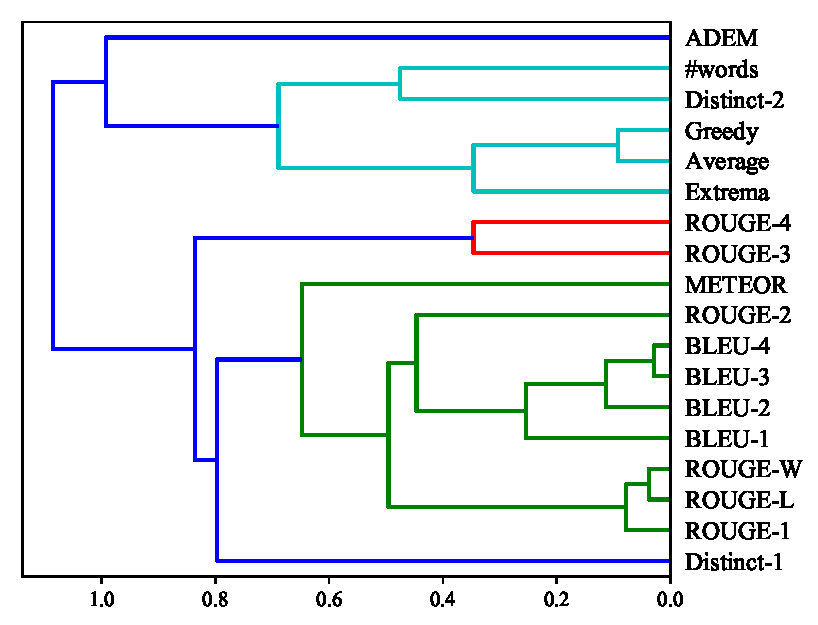
\includegraphics[width=\linewidth]{figure/plot/hierarchy/v3/pearson/hred/ubuntu/plot.pdf}
        \caption{(HRED, Ubuntu)}
    \end{subfigure}
    \begin{subfigure}{0.35\linewidth}
        \centering
        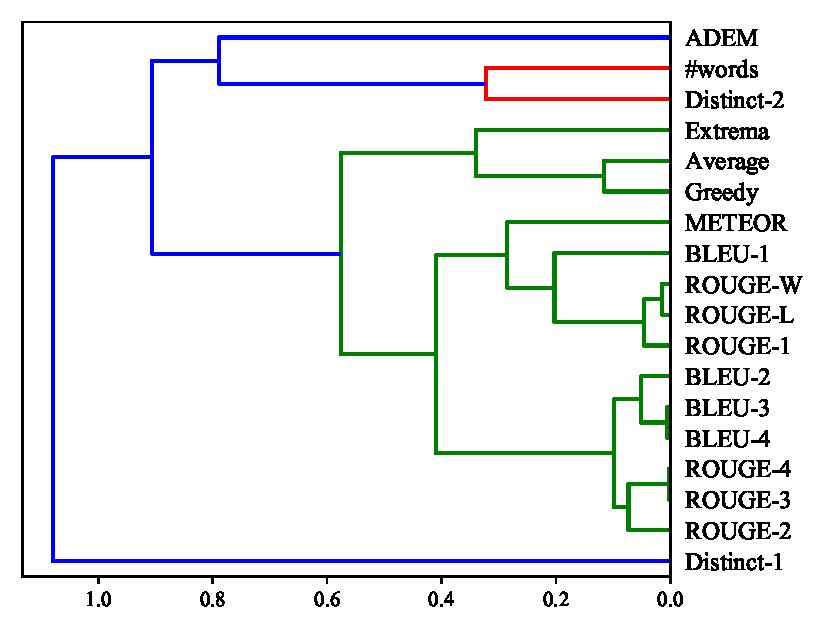
\includegraphics[width=\linewidth]{figure/plot/hierarchy/v3/pearson/vhred/lsdscc/plot.pdf}
        \caption{(VHRED, LSDSCC)}
    \end{subfigure}%
    \begin{subfigure}{0.35\linewidth}
        \centering
        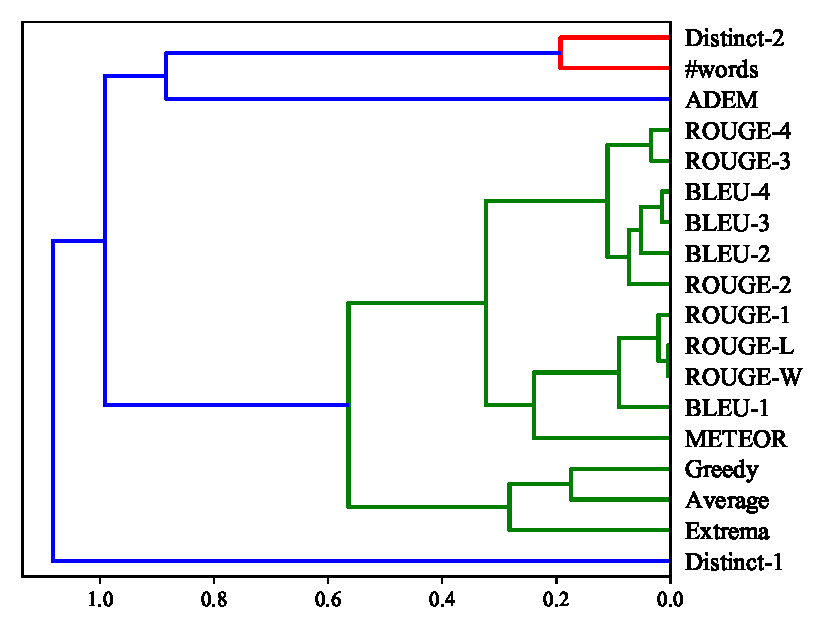
\includegraphics[width=\linewidth]{figure/plot/hierarchy/v3/pearson/vhred/opensub/plot.pdf}
        \caption{(VHRED, OpenSubtitles)}
    \end{subfigure}%
    \begin{subfigure}{0.35\linewidth}
        \centering
        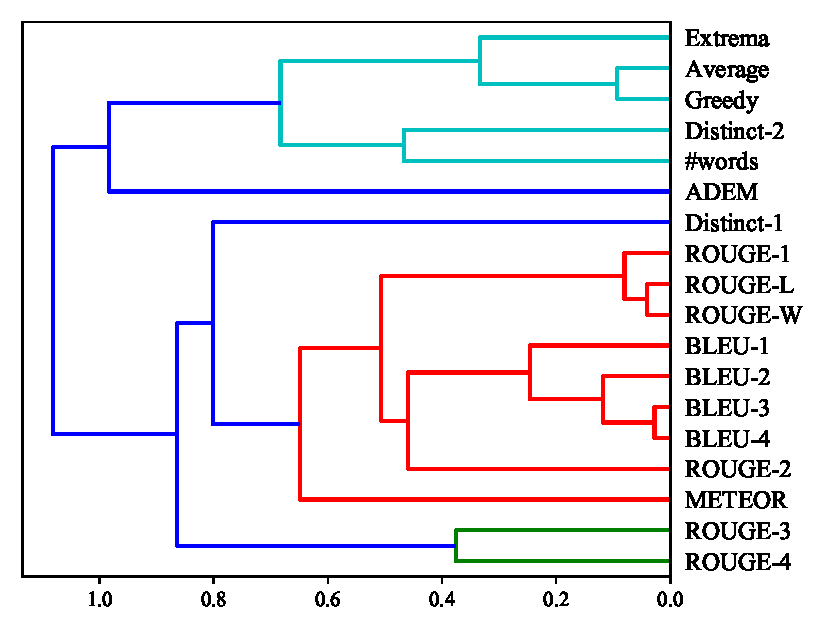
\includegraphics[width=\linewidth]{figure/plot/hierarchy/v3/pearson/vhred/ubuntu/plot.pdf}
        \caption{(VHRED, Ubuntu)}
    \end{subfigure}
    \begin{subfigure}{0.35\linewidth}
        \centering
        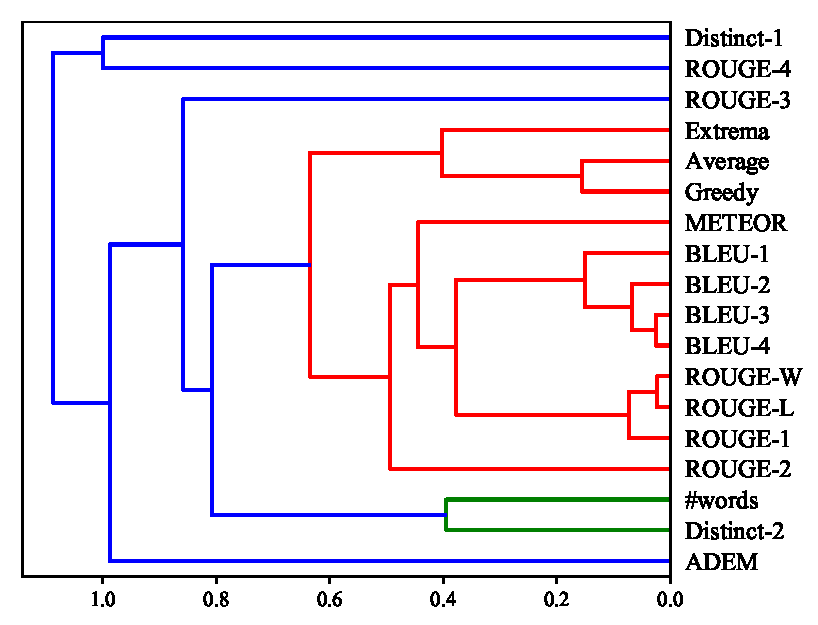
\includegraphics[width=\linewidth]{figure/plot/hierarchy/v3/pearson/lstm/lsdscc/plot.pdf}
        \caption{(LSTM, LSDSCC)}
    \end{subfigure}%
    \begin{subfigure}{0.35\linewidth}
        \centering
        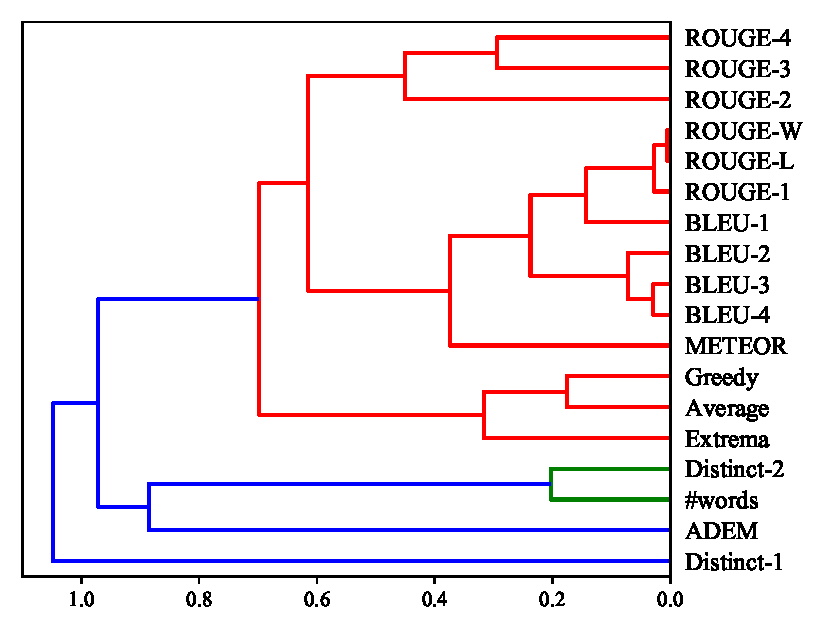
\includegraphics[width=\linewidth]{figure/plot/hierarchy/v3/pearson/lstm/opensub/plot.pdf}
        \caption{(LSTM, OpenSubtitles)}
    \end{subfigure}%
    \begin{subfigure}{0.35\linewidth}
        \centering
        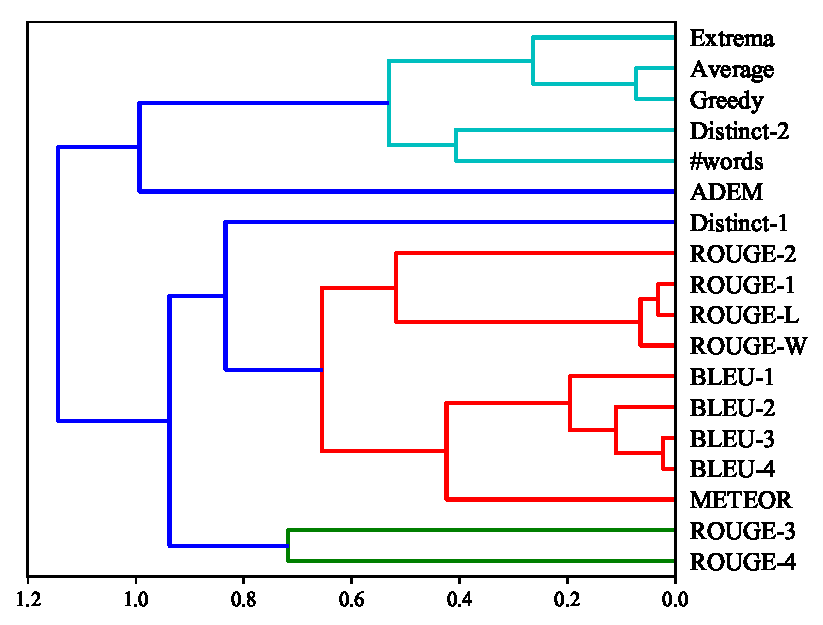
\includegraphics[width=\linewidth]{figure/plot/hierarchy/v3/pearson/lstm/ubuntu/plot.pdf}
        \caption{(LSTM, Ubuntu)}
    \end{subfigure}
    \centering
    \caption{Hierarchical Clusterings with Pearson's r}
    \label{fig:hierarchy}
\end{figure}
